\chapter{Literatuurstudie}
\label{ch:literatuurstudie}

% Tip: Begin elk hoofdstuk met een paragraaf inleiding die beschrijft hoe
% dit hoofdstuk past binnen het geheel van de bachelorproef. Geef in het
% bijzonder aan wat de link is met het vorige en volgende hoofdstuk.

% Pas na deze inleidende paragraaf komt de eerste sectiehoofding.

In dit hoofdstuk wordt er meer achtergrondinformatie gegeven. Het hoofdstuk start met extra informatie over mobile coaching apps. Daarna worden onderzoeken die in het verleden zijn gedaan naar mobile coaching bestudeerd. 

\section{Stand van zaken in het onderzoeksdomein}
\label{sec:stand-van-zaken}

Door de grote opkomst van smartphones, zijn er al enkele onderzoeken gedaan naar gezondheidsapplicaties. Deze studies stellen de kwaliteit van de applicaties in vraag. In de onderzoeken gaan ze na of het gebruik van dergelijke apps wel een positief effect heeft op de gezondheid van de mensen. 

Er zijn ook onderzoeken in dit domein die de evolutie van gezondheidsapplicaties bestuderen en bekijken hoe we in de toekomst nog betere applicaties kunnen maken. In 2013 ~\autocite{Wikipedia2013} was er een nieuwe trend, namelijk de smartwatch. Vanaf dan ging deze markt in een stroomversnelling en werd integratie met applicaties mogelijk. Applicatie ontwikkelaars hadden dus een nieuwe functie om als eerste op in te spelen. 
\newpage

\section{Werking van mobile coaching applicaties}
\label{sec:werking}

Mobile coaching applicaties werken praktisch altijd op dezelfde manier. Een gebruiker of een apparaat ( bv. Een smartwatch) levert input  zoals aantal stappen, aantal uren slaap, hartslagfrequentie, gepresteerde oefening of gegeten voeding. De applicatie kan verder aan de slag met de data te verwerken. Sommige van deze applicaties hebben ook een extra functie waardoor je externe apps kunt koppelen aan jouw coaching applicatie. Bijvoorbeeld kan Myfitnesspal gekoppeld worden met stappentellers en trainingsapplicaties. De calorieteller houdt dan rekening met de beweging van de gebruiker die dag en deze calorieën worden dan in vermindering gebracht. 

Stappentellers zijn hier een uitstekend voorbeeld van. Maar over het algemeen dient de gebruiker zelf aan de applicatie te vertellen wat hij of zij gedaan heeft. Het is afhankelijk van applicatie tot applicatie wat je precies allemaal kunt invoeren. 

De data wordt meestal in de cloud opgeslagen zodat deze toegankelijk wordt op alle toestellen van de gebruiker. Zo kan de gebruiker ook z’n resultaten bekijken op de computer door zich aan te melden op het online platform.

Mobile coaching applicaties komen volledig tot hun recht als gebruikers alle gegevens elke dag of trainingsdag bijhouden in de app. Dan kan de gebruiker na verloop van tijd z’n eigen progressie zien en analyses maken op de data van het verleden.

In onderstaande afbeelding wordt de algemene werking van een mobile coaching applicatie geïllustreerd. De gebruiker draagt een smartwatch die input levert samen met de smartphone. 

De data wordt allemaal gesynchroniseerd in de cloud zodat dit op elk moment kan opgevraagd worden door een ander apparaat die ook verbonden is met het account van de gebruiker

\begin{figure}[h!]
\centering
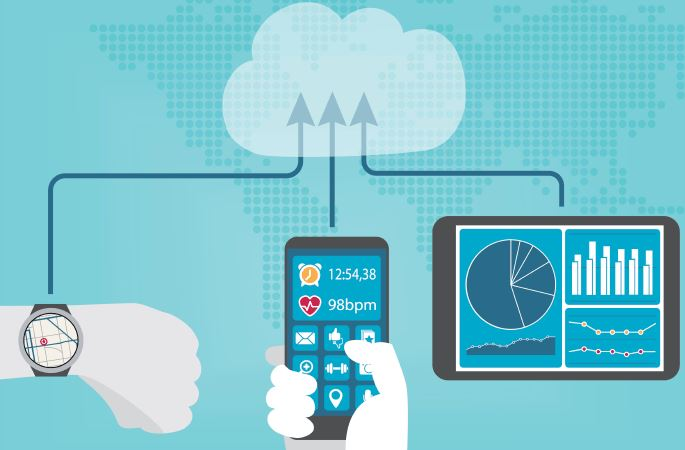
\includegraphics[width=0.7\textwidth]{img/cloud-synch.JPG}
\caption{werking mobile coaching apps (patientengagementhit.com,2017)}
\end{figure}

\newpage
\section{Verschillende types mobile coaching applicaties}
\label{sec:types}

Er zijn verschillende types mobile coaching applicaties waaruit je kan kiezen. In dit onderzoek is gekozen om de volgende 3 rubrieken te onderzoeken omdat er tussen deze types een significant verschil is:

\begin{itemize}
\setlength\itemsep{1em}
\item {\bf Voedingsapplicaties:} Deze applicaties begeleiden gebruikers alleen op het vlak van dieet en voeding. Dergelijke apps werken met een puntensysteem of met calorieën zodat gebruikers ofwel gewicht kunnen aankomen of afvallen, dit is natuurlijk afhankelijk van het doel van de gebruikers.

\item {\bf Trainingsapplicaties:} leiden tot schema’s die gebruikers zullen volgen bij hun training. Het schema zal vooraf worden ingesteld met het doel van de gebruiker bijvoorbeeld intensiteit of niveau van de oefeningen op het trainingsschema.

\item {\bf Coaching applicaties:} steunen de gebruikers door de dag heen grotendeels op gebied van training. Daarbij zal dit type applicaties ook fungeren als een virtuele coach die je nog extra motiveert om te bewegen. Als je niet aan je dagelijkse behoefte zit, dan zul je meldingen op je smartphone ontvangen enzovoort. Deze applicaties focussen zich niet alleen fysisch maar ook mentaal. Deze apps dienen als centraal punt voor alle andere bewegingsapps, ze verzamelen zoveel mogelijk data om de gebruiker zo efficiënt mogelijk te helpen.

\end{itemize}

\section{Vergelijkbare onderzoeken}
\label{sec:vergelijkbare-onderzoeken}

In dit onderdeel zullen vergelijkbare onderzoeken toegelicht worden. Er zal telkens een korte inhoud geschetst worden. 

\subsection{Hoe maak je betere fitness applicaties}
\label{sec:betere-apps}

Eerst wordt een artikel van The App Solutions \autocite{TheAppSolutions2017} bekeken die algemeen beschrijft hoe een ideale fitness app is opgebouwd. Zij verdelen de applicaties in 3 categorieën. Deze 3 categorieën zijn ook gekozen in dit onderzoek. De beschrijvingen van alle categorieën zijn ter verduidelijking.

\begin{itemize}
\setlength\itemsep{1em}
\item {\bf Dieet – en voedingsapplicaties:  } helpen gebruikers om zicht te krijgen op hun eetpatroon. Meestal maken dergelijk applicaties gebruik van calorieën. De gebruiker geeft zelf in wat er per maaltijd gegeten wordt. De applicatie herkent het product meestal en berekent zo de calorieën. Gebruikers stellen zelf hun limiet in door een doel te selecteren ( bijvoorbeeld ‘afvallen’) en de applicatie zegt hoeveel je mag en kan eten om het doel te bereiken.

Gegeven tips voor dit type: Het integreren van een boodschappenlijstje met suggesties voor recepten. Zo kunnen gebruikers makkelijker inschattingen maken. Bovendien helpen ze ook bij het maken van keuzes in de supermarkt. Het voorzien van een barcode scanner zodat gebruikers makkelijk hun voeding kunnen terugvinden in de database van de applicatie. Het versnelt ook het proces waardoor gebruikers minder moeite moeten doen om hun etenswaren te vinden.

\item {\bf Apps die gebruikt worden als activiteiten logboek (Mobile coaching) : } De applicaties kunnen zowel automatisch fysische activiteiten registreren door sensors in smartphones of als de gebruiker manueel zijn activiteit ingeeft. Dit type applicaties is handig om vooruitgang te zien omdat ze de mogelijkheid bieden om grafieken te genereren van prestaties in het verleden.

Gegeven tips voor dit type: Voor de gebruikers is het praktischer om een account te kunnen aanmaken omdat ze op die manier de mogelijkheid krijgen om de prestaties op andere toestellen te bekijken zoals tablet of computer. Tegenwoordig heeft bijna iedere sporter een smartwatch dus het is handig om deze te integreren in de applicatie, hierdoor moeten gebruikers ook zelf minder data manueel ingeven. Sociale media is een populair middeltje om gebruikers hun prestaties te laten delen met de buitenwereld. Het zorgt overigens voor publiciteit van de gebruikte applicatie en het kan dienen als extra motivatie voor de gebruiker als ze steun krijgen van vrienden. Geolocatie bepaalt de positie van de gebruiker door middel van een GPS-signaal. Daardoor kunnen gebruikers routes terug bekijken als ze dat wensen. Een laatste tip zijn push noticataties. Deze notificaties verschijnen als melding op het hoofdscherm van de smartphone. Ze zorgen ervoor dat gebruikers worden aangemoedigd en herinnerd om te bewegen.
\item {\bf  Fitness applicaties:  } Deze applicaties zorgen ervoor dat gebruikers makkelijker een eigen trainingsschema kunnen samenstellen. Als gebruikers de applicatie voor het eerst opstarten dan doorloopt de applicatie een aantal vragen en op basis van het antwoord wordt dan een trainingsschema gegenereerd.
Gegevens tips voor dit type zijn niet gespecifieerd in dit artikel. Meest van bovenstaande tips zijn hier ook van toepassing. 
\end{itemize}

\subsection{Onderzoek naar kwaliteit van mobile coaching applicaties met ACSM-richtlijnen}
\label{sec:onderzoek-ACSM-richtlijnen}

In het artikel van University of Florida \autocite{mhealth2015} bestuderen ze de kwaliteit van mobile coaching applicaties die op dat moment op de markt waren. Ze beschrijven de opmars van de smartphone in combinatie met de talloze apps die gebruikers kunnen installeren. Echter zijn er geen controles op de kwaliteit van applicaties die te downloaden zijn en daar gaat het artikel over. Ze willen de kwaliteit van de applicaties zelf gaan beoordelen.

In het onderzoek wordt enkel gebruik gemaakt van IOS-applicaties. Dit begrenst enigszins de mogelijkheden van het onderzoek. In de Apple store werden 30 applicaties gedownload en vervolgens werden deze getest met richtlijnen van ACSM (American College of Sports Medicine).
Elke geteste applicatie kreeg een score die gebaseerd was op een aantal subgroepen: flexibiliteit ( 0 tot 2 puntent) , aerobe (0-6 punten), weerstand ( 0 tot 6 punten). In totaal was er dus een score op 14 per applicatie.

Volgens de resultaten van het onderzoek had maar 1 applicatie een totale score boven de 50\%. Uit het onderzoek is dus besloten dat er slecht een klein aantal apps aan de kwaliteitsnormen voldoen. In dit geval zijn het wel specifieke richtlijnen uit Amerika. Deze studie bewijst ook dat dus maar een klein procent van de applicaties effectief helpen om gewicht te verliezen of om een ander doel te bereiken. Applicatie ontwikkelaars hebben dus een grote mogelijkheid om de kwaliteit enorm te verbeteren.

\subsection{Mobiele gezondheidsapplicaties geïndentificeerd volgens RTC}
\label{sec:onderzoek-RTC}

In het artikel van Digital Medicine \autocite{DigitalMedicine2015} zijn 22 applicaties beoordeeld waarbij de focus op obesitas, diabetisch \& mentale gezondheid ligt. Het onderzoek is getest met de RTC-methode (Randomized Controlled Trial). Dit houdt in dat de geteste stelling, in dit geval de 3 focuspunten van het onderzoek,  wordt uitgevoerd op een interventie groep en dat resultaat wordt vergeleken met een controlegroep. Het onderzoek heeft als doel de effectiviteit van mobiele gezondheidsapplicaties beoordelen.

Digital Medicine beveelt ontwikkelaars aan om voor de release van de applicatie, uitvoerig te testen. Dit kan vele fouten vermijden en zal de effectiviteit verbeteren.

\section{Gekozen applicaties}
\label{sec:gekozen-apps}
In dit onderdeel zal er voor elke gekozen categorie, 2 tot 3 applicaties gekozen worden. De gekozen applicaties zijn bekende applicaties met een hoog aantal downloads volgens Appbrain \autocite{Appbrain2018}. Er zullen nog geen conclusies getrokken worden, de applicaties worden enkel kort voorgesteld. Op basis van de enquête en vooraf bepaalde kritische punten, zal later in dit onderzoek de beste applicatie volgens de bepaalde kritische punten gekozen worden.

\subsection{Voedingsapplicaties}
\label{sec:Voedingsapplicaties}
\textbf{MyFitnessPal}

MyFitnesspal laat bezoekers toe om een voedingslogboek bij te houden zodat je zicht krijgt op je goede en minder goede gewoontes. De app biedt ook de mogelijkheid om met andere apps te interageren zodat gebruikers zelf minder input moeten leveren. Myfitnesspal werkt hoofdzakelijk met het berekenen van calorieën. Op die manier kan de gebruiker ook zicht krijgen op hoeveel calorieën hij die dag heeft verbrand. 

Er is ook een premium versie van de applicatie die extra functionaliteiten aanbiedt zoals: exclusieve recepten, extra overzichtelijk dashboard en advertentievrij.
Deze applicatie is beschikbaar op zowel Android als IOS.
\newpage
Functies in de gratis versie:
\begin{itemize}

    \item Dagelijks caloriedoel instellen
    \item Kies uw patroon volgens macro’s ( Koolhydraten, eiwitten \& vetten)
    \item Voeg snel uw gegeten voeding toe door de zoekfunctie + barcode scanner
    \item Rapporten beschikbaar door middel van grafieken
    \item Verbind andere fitness apps om calorieverbruik te volgen
\end{itemize}

\textbf{Lose It!}

Lose it! legt de klemtoon ook op het tellen van calorieën. De applicatie is volgens de makers heel makkelijk en aantrekkelijk.

De applicatie biedt ook een premium versie aan die gebruikers toelaat om doelen in te stellen voor bepaalde voedingstypes ( bijvoorbeeld het halen van een vitamine doel).
De app is ook beschikbaar op IOS en Android.

Functies in de gratis versie:
\begin{itemize}
\item Dagelijks caloriedoel instellen
\item Scan voeding met de barcode scanner
\item Neem een foto van voeding en de app herkent dit
\item Rapporten beschikbaar door middel van grafieken
\item Toegang tot de community 
\end{itemize}


\textbf{FatSecret}

Fatsecret is volledig gratis. De makers noemen het de snelste en makkelijkste calorieteller. Fatsecret maakt gebruik van de community om beter te worden. 

De app is beschikbaar op IOS en Android.

Functies:
\begin{itemize}
\item Voedingsdagboek
\item Gezonde recepten
\item Voedingsinfo voor alle soorten voeding
\item Oefeningendagboek om verbranding van calorieën bij te houden
\item Rapporten beschikbaar door middel van grafieken
\end{itemize}

\newpage
\subsection{Trainingsapplicaties}
\label{sec:Trainingsapplicaties}


\textbf{Total Fitness - Gym \& Workouts}

Total Fitness biedt gebruikers veel informatie over oefeningen om gebruikers hun doel te laten bereiken. Oefeningen worden uitgebreid uitgelegd. De oefeningen kunnen zowel voor thuis als in de fitness zijn.
Deze app is beschikbaar op IOS en Android.


Functies:
\begin{itemize}
\item Begeleide trainingen
\item Trainingbouwer
\item Stel uitdagingen in
\end{itemize}

\textbf{Fitnessuitdaging in 30 dagen}

De applicatie biedt trainingen om thuis te doen. Gebruikers kunnen de intensiteit van de oefeningen stap per stap verhogen. De applicatie is bedoeld voor beginners maar ook gevorderde gebruikers.
Deze app is beschikbaar op IOS en Android.

Functies:
\begin{itemize}
\item Registeren van progressie van de gebruiker
\item Videogids
\item Sociale media integratie
\item Oefeningen voor het volledige lichaam, buikspieren en benen 
\end{itemize}

\textbf{Workouts voor thuis}

Deze app biedt dagelijkse trainingsroutines voor alle spiergroepen. Het grote voordeel van deze applicatie is dat je geen fitnessabonnement en dure apparatuur moet hebben. Alle oefeningen zijn gebasseerd op lichaamsgewicht.
Deze app is beschikbaar op IOS en Android.

Functies:
\begin{itemize}
\item Warm-up en stretch oefeningen
\item Registreren van progressie
\item Videobegeleiding
\item Sociale media integratie
\end{itemize}

\subsection{Coaching applicaties}
\label{sec:Coachingapplicaties}

\textbf{Google Fit}

Google Fit laat gebruikers hun fitnessdoelen bereiken door aangepaste coaching in combinatie met tips. De tips zijn gebasseerd op de gezondheid van de gebruikers en het activiteiten logboek. De app werkt met bewegings- en hartpunten. 

Deze punten verdien je stelselmatig door de dag heen. Hartpunten verdient de gebruikers als de hartslag omhoog gaat, bij intense schommelingen krijgt de gebruiker dubbele punten. Deze punten dienen vooral voor de mentale gezondheid van de gebruiker te coachen.
Google Fit is enkel beschikbaar op Android.

Functies:
\begin{itemize}
\item Integratie van andere fitness apps is mogelijk
\item Integratie van smartwatches
\item Focus op gewicht, beweging, calorieën en slaap
\item Vooruitgang visualiseren                                                          
\end{itemize}

\textbf{Apple Health}

Apple Health legt de focus hoofdzakelijk op fysieke en mentale gezondheid van de gebruikers. De applicatie verzamelt gegevens uit allerhande apps. Deze applicatie dient dan als centraal punt waar de gebruiker al zijn verzamelde gegevens kan bekijken.

De applicatie kent 4 categorieën: activiteit, slaap , mindfullness en voeding. De app meet automatisch het aantal stappen of de afstand van punt a naar b. De mindfullness-functie is iets bijzonder omdat de focus volledig op de mentale gezondheid ligt, even aan niets denken kan wonderen doen. De applicatie is enkel beschikbaar voor IOS.

Functies:
\begin{itemize}
\item Integratie van andere fitness apps mogelijk
\item Integratie van smartwatches
\item Focus op mentale en fysieke gezondheid
\item Duidelijke overzichten
\end{itemize}
